%%%%%%%%%%%%%%%%%%%%%%%%%%%%%%%%%%%%%%%%%%%%%%%%%%%%%%%%%%%%%%%%%%%%%%%%%%%
%
% Generic template for TFC/TFM/TFG/Tesis
%
% $Id: resultados.tex,v 1.7 2016/03/31 10:44:23 macias Exp $
%
% By:
%  + Javier Macías-Guarasa.
%    Departamento de Electrónica
%    Universidad de Alcalá
%  + Roberto Barra-Chicote.
%    Departamento de Ingeniería Electrónica
%    Universidad Politécnica de Madrid
% 
% Based on original sources by Roberto Barra, Manuel Ocaña, Jesús Nuevo, Pedro Revenga, Fernando Herránz and Noelia Hernández. Thanks a lot to all of them, and to the many anonymous contributors found (thanks to google) that provided help in setting all this up.
%
% See also the additionalContributors.txt file to check the name of additional contributors to this work.
%
% If you think you can add pieces of relevant/useful examples, improvements, please contact us at (macias@depeca.uah.es)
%
% You can freely use this template and please contribute with comments or suggestions!!!
%
%%%%%%%%%%%%%%%%%%%%%%%%%%%%%%%%%%%%%%%%%%%%%%%%%%%%%%%%%%%%%%%%%%%%%%%%%%%

\chapter{Resultados experimentales y análisis comparativo}
\label{cha:resultados}

\section{Introducción}

Una vez descrito el marco metodológico y completado el proceso de entrenamiento e inferencia de los distintos modelos evaluados, este capítulo presenta los resultados experimentales obtenidos y su análisis comparativo. El objetivo principal es estudiar el comportamiento de los modelos \ac{BERT}, los \acp{LLM} open-source y los \acp{LLM} comerciales avanzados sobre la tarea de detección de trastornos de salud mental, permitiendo identificar tanto sus fortalezas como sus limitaciones en distintos escenarios de clasificación.

Con el fin de facilitar la interpretación, el capítulo se organiza por tareas: ansiedad, depresión, \ac{TCA} y clasificación multiclase. Para cada una de ellas se sigue la misma estructura de análisis, comenzando por las métricas principales de rendimiento y estabilidad predictiva, continuando con el estudio cualitativo mediante matrices de confusión, la comparación estadística entre modelos mediante bootstrap pareado y, finalmente, el análisis de la relación entre rendimiento y coste computacional.

Esta organización permite no solo comparar qué modelos obtienen mejores resultados en cada tarea concreta, sino también comprender cómo varía su comportamiento según el tipo de trastorno analizado y el equilibrio existente entre precisión, robustez inferencial y eficiencia práctica.

\section{Clasificación de ansiedad}

\subsection{Métricas principales y estabilidad predictiva}
La Tabla~\ref{tab:resultados_ansiedad_metricas} recoge los resultados obtenidos en la tarea de clasificación de ansiedad, incluyendo las métricas principales de rendimiento (F1-score macro, Precision, Recall y \ac{MCC}) junto con sus intervalos de confianza al 95\% estimados mediante bootstrap \ac{BCa}, así como la consistencia predictiva medida mediante \ac{TARa@5}. En cada celda se muestra el valor de la métrica y, entre corchetes, los límites inferior y superior del intervalo de confianza correspondiente.

\begin{table}[H]
	\centering
	\caption{Resultados principales en la tarea de clasificación de ansiedad}
	\label{tab:resultados_ansiedad_metricas}
	\resizebox{\textwidth}{!}{
		\begin{tabular}{lccccc}
			\toprule
			\textbf{Modelo} & \textbf{F1 macro} & \textbf{Precision} & \textbf{Recall} & \textbf{MCC} & \textbf{TARa@5} \\
			\midrule
			DistilBETO & 0.650 [0.476, 0.823] & 0.670 [0.458, 0.873] & 0.636 [0.478, 0.835] & 0.305 [-0.056, 0.644] & -- \\
			RoBERTa-large-BNE & 0.680 [0.529, 0.830] & 0.660 [0.531, 0.811] & 0.717 [0.527, 0.880] & 0.373 [0.073, 0.658] & -- \\
			mDeBERTa-v3 & 0.593 [0.460, 0.791] & 0.616 [0.443, 0.897] & 0.581 [0.470, 0.798] & 0.194 [-0.079, 0.572] & -- \\
			Longformer & 0.468 [0.440, 0.486] & 0.440 [0.393, 0.473] & 0.500 [0.500, 0.500] & 0.000 [0.000, 0.000] & -- \\
			\midrule
			Llama 3.1 8B & 0.711 [0.642, 0.788] & 0.856 [0.759, 0.927] & 0.661 [0.604, 0.729] & 0.479 [0.346, 0.613] & 0.980 [0.959, 0.992] \\
			GPT-OSS-20B & 0.840 [0.780, 0.891] & 0.932 [0.857, 0.965] & 0.786 [0.726, 0.850] & 0.703 [0.597, 0.794] & 0.988 [0.970, 0.996] \\
			DeepSeek-V3.2 & 0.739 [0.677, 0.794] & 0.713 [0.653, 0.769] & 0.778 [0.714, 0.840] & 0.487 [0.368, 0.595] & 0.988 [0.961, 0.996] \\
			Claude Sonnet 4.6 & 0.805 [0.732, 0.862] & 0.909 [0.830, 0.951] & 0.750 [0.679, 0.815] & 0.640 [0.514, 0.740] & 0.994 [0.984, 0.998] \\
			GPT-5.2 & 0.820 [0.757, 0.878] & 0.915 [0.838, 0.957] & 0.767 [0.701, 0.831] & 0.666 [0.547, 0.766] & 0.998 [0.990, 1.000] \\
			Gemini 3.1 Pro & 0.815 [0.758, 0.869] & 0.813 [0.746, 0.875] & 0.818 [0.757, 0.879] & 0.631 [0.516, 0.737] & 0.990 [0.978, 0.996] \\
			\bottomrule
		\end{tabular}
	}
\end{table}

De forma general, los resultados muestran una superioridad clara de los \acp{LLM} frente a los modelos BERT tradicionales.

El mejor resultado global corresponde a GPT-OSS-20B, que obtiene el mayor F1-score macro (0.840), así como los mejores valores de Precision (0.932), Recall (0.786) y \ac{MCC} (0.703). Esto indica no solo una mayor capacidad predictiva general, sino también un mejor equilibrio entre clases y una clasificación más robusta frente al desbalance del dataset. Aunque su valor de \ac{TARa@5} (0.988) es ligeramente inferior al de algunos modelos propietarios como GPT-5.2 o Claude, sigue representando una consistencia predictiva muy elevada.

En el grupo de modelos propietarios, GPT-5.2, Claude Sonnet 4.6 y Gemini 3.1 Pro presentan resultados muy próximos entre sí, con valores de F1 macro superiores a 0.80 y \ac{TARa@5} cercanos a 1. Esto refleja una gran estabilidad en la inferencia incluso bajo múltiples ejecuciones. DeepSeek-V3.2, sin embargo, muestra un comportamiento inferior dentro de este grupo, con un F1-score macro de 0.739 y un rendimiento más cercano al observado en Llama 3.1 8B que al resto de modelos frontier.

Dentro de los modelos BERT, el comportamiento es considerablemente más débil. Aunque RoBERTa-large-BNE obtiene el mejor resultado de este grupo (F1 = 0.680), todos los modelos muestran dificultades para manejar adecuadamente el desbalance entre clases, previamente observado en la Figura~\ref{fig:dist_clases_mentalriskes}. Esta situación resulta especialmente evidente en Longformer, cuyo Recall de 0.500 y \ac{MCC} igual a 0 sugieren un comportamiento prácticamente equivalente a predecir siempre la clase mayoritaria. En este caso, el modelo tiende a clasificar sistemáticamente los ejemplos como ansiedad (\texttt{1}), reduciendo drásticamente su capacidad discriminativa frente a la clase control (\texttt{0}).

\subsection{Análisis de errores mediante matrices de confusión}

El análisis de las matrices de confusión de todos los modelos evaluados muestra un patrón común en la tarea de clasificación de ansiedad: la mayoría presentan un sesgo hacia la clase positiva, priorizando la detección de casos de ansiedad frente a la correcta identificación de usuarios control. Este comportamiento incrementa el \textit{recall}, al reducir los falsos negativos, pero también genera un mayor número de falsos positivos, afectando negativamente a la precisión y dificultando una separación más equilibrada entre ambas clases.

Para facilitar la interpretación, en la Figura~\ref{fig:cm_ansiedad} se presentan tres casos representativos: el mejor resultado global (GPT-OSS-20B), el mejor modelo BERT (RoBERTa-large-BNE) y un caso especialmente ilustrativo de fallo sistemático (Longformer). El conjunto completo de matrices de confusión de todos los modelos evaluados se incluye en el Anexo~\ref{anexo:mc_anx}, con el fin de no sobrecargar la presentación principal de resultados.

\begin{figure}[H]
	\centering
	
\includegraphics[width=\textwidth]{cm_ansiedad.png}
	\caption{Matrices de confusión representativas en la tarea de clasificación de ansiedad}
	\label{fig:cm_ansiedad}
\end{figure}

\begin{itemize}
	
	\item GPT-OSS-20B: Presenta el mejor equilibrio general entre ambas clases. Mantiene una detección casi perfecta de usuarios con ansiedad (99.3\%), al mismo tiempo que mejora de forma notable la identificación de la clase control frente al resto de modelos, aunque todavía conserva una cierta tendencia a generar falsos positivos (42.1\%).
	
	\item RoBERTa-large-BNE: Muestra un comportamiento similar, pero con menor capacidad discriminativa. Aunque detecta correctamente la mayoría de los casos positivos (87.9\%), incrementa tanto los falsos negativos como los falsos positivos respecto a GPT-OSS-20B, reflejando las limitaciones de los modelos BERT ante el desbalance de clases.
	
	\item Longformer: Representa el caso más extremo, ya que clasifica el 100\% de los ejemplos como ansiedad (\texttt{1}), sin identificar correctamente ningún usuario control. Esto explica directamente su \ac{MCC} igual a cero y confirma que el modelo ha aprendido únicamente a reproducir la clase mayoritaria.
	
\end{itemize}

En conjunto, las matrices de confusión refuerzan la interpretación obtenida a partir de las métricas globales y permiten visualizar con mayor claridad cómo los mejores resultados no dependen únicamente de un F1-score elevado, sino también de la capacidad real del modelo para discriminar correctamente entre ambas clases sin sesgarse excesivamente hacia la clase positiva.

\subsection{Comparación y significancia estadística entre modelos}

Para complementar la tabla principal de métricas, se realizó una comparación estadística entre modelos mediante bootstrap pareado utilizando F1 macro como métrica principal. Esta comparación permite no solo observar qué modelo obtiene mejor rendimiento, sino también comprobar si dichas diferencias son suficientemente consistentes como para considerarse estadísticamente significativas y si, además, presentan una magnitud práctica relevante.

Dado que comparar todos los modelos entre sí generaría un número excesivo de combinaciones y dificultaría la interpretación, se seleccionaron únicamente los modelos más representativos de cada grupo: el mejor modelo BERT, el mejor LLM open-source y los dos mejores LLMs propietarios. Para garantizar comparaciones homogéneas, todas las pruebas se realizaron sobre exactamente el mismo subconjunto común de ejemplos.

La Tabla~\ref{tab:bootstrap_ansiedad} muestra, para cada par de modelos, la diferencia media de F1 macro (\textit{Mean $\Delta$}), junto con su intervalo de confianza del 95\%, el tamaño del efecto mediante Cohen’s \(d\), acompañado de su interpretación cualitativa (\textit{Effect size}) y el \textit{p-value} ajustado mediante corrección de Benjamini-Hochberg (BH). Una diferencia media positiva indica mejor rendimiento del Modelo A, mientras que una diferencia negativa favorece al Modelo B.

Este mismo procedimiento se aplicará posteriormente en las tareas de depresión, TCA y clasificación multiclase, manteniendo siempre el mismo criterio de selección para garantizar comparaciones homogéneas.

\begin{table}[H]
	\centering
	\small
	\begin{tabular}{llllll}
		\hline
		\textbf{Model A} & \textbf{Model B} & \textbf{Mean $\Delta$} & \textbf{Cohen's d} & \textbf{Effect size} & \textbf{\textit{p}} \\
		\hline
		RoBERTa-large-BNE & GPT-OSS-20B & -0.220 [-0.385, -0.051] & -2.566 & Large & 0.072 \\
		RoBERTa-large-BNE & GPT-5.2 & -0.109 [-0.289, 0.105] & -1.060 & Large & 0.360 \\
		RoBERTa-large-BNE & Gemini 3.1 Pro & -0.109 [-0.310, 0.085] & -1.059 & Large & 0.360 \\
		GPT-OSS-20B & GPT-5.2 & 0.111 [-0.026, 0.314] & 1.326 & Large & 0.352 \\
		GPT-OSS-20B & Gemini 3.1 Pro & 0.111 [0.000, 0.271] & 1.692 & Large & 0.306 \\
		GPT-5.2 & Gemini 3.1 Pro & 0.000 [-0.212, 0.140] & -0.020 & Negligible & 0.980 \\
		\hline
	\end{tabular}
	\caption{Comparación estadística mediante bootstrap pareado para la tarea de ansiedad.}
	\label{tab:bootstrap_ansiedad}
\end{table}

La comparación más relevante se observa entre RoBERTa-large-BNE y GPT-OSS-20B, donde la diferencia media de rendimiento favorece claramente al modelo open-source, lo que indica una mejora apreciable de GPT-OSS-20B respecto al mejor modelo BERT. Además, el intervalo de confianza no incluye el cero, lo que sugiere una diferencia consistente. Esta comparación presenta además un tamaño del efecto elevado ($d = -2.566$) clasificado como \textit{Large}, lo que indica que la mejora no solo existe, sino que resulta relevante desde un punto de vista práctico. Sin embargo, tras aplicar la corrección de Benjamini-Hochberg, el p-value ajustado alcanza $p = 0.072$ por lo que la comparación no alcanza el umbral convencional de significancia estadística ($p < 0.05$), aunque sí muestra una tendencia clara hacia la superioridad de GPT-OSS-20B.

En el resto de comparaciones, los p-values son considerablemente más altos y los intervalos de confianza incluyen el cero, indicando ausencia de evidencia estadística suficiente para afirmar diferencias robustas entre modelos. Esto ocurre especialmente entre los tres modelos con mejor rendimiento global (GPT-OSS-20B, GPT-5.2 y Gemini 3.1 Pro), cuyos resultados son muy próximos entre sí.

Por ejemplo, la comparación entre GPT-5.2 y Gemini 3.1 Pro presenta una diferencia prácticamente nula ($\Delta = 0.000 \quad [-0.212,\ 0.140]$) acompañada de un tamaño del efecto prácticamente inexistente ($d = -0.020$) clasificado como \textit{Negligible}, lo que confirma que ambos modelos presentan un comportamiento prácticamente equivalente en esta tarea. El p-value ajustado de $p = 0.980$ refuerza esta interpretación, indicando ausencia total de evidencia estadística de superioridad entre ambos sistemas.

En conjunto, estos resultados indican que, aunque los LLMs muestran mejores métricas agregadas que los modelos BERT, en la tarea de ansiedad las diferencias entre los mejores sistemas no siempre son suficientemente robustas desde el punto de vista estadístico. El caso de GPT-OSS-20B frente a RoBERTa-large-BNE sugiere una mejora clara tanto en rendimiento como en tamaño del efecto, pero sin alcanzar significancia formal tras la corrección por comparaciones múltiples.

\subsection{Análisis rendimiento-coste}

Además del rendimiento predictivo, resulta relevante analizar hasta qué punto las mejoras obtenidas por cada modelo justifican el coste computacional necesario para alcanzarlas. Para ello, se representa un diagrama de eficacia frente a coste, donde el eje X muestra el coste estimado de cada modelo para la tarea evaluada y el eje Y su rendimiento en términos de F1 macro.

En el caso de los modelos BERT, el coste se estimó a partir del tiempo total de entrenamiento e inferencia utilizando una GPU de pago\footnote{Aunque los experimentos se ejecutaron sobre una GPU NVIDIA T4 en Google Colab gratuito, para estimar el coste en un entorno reproducible y comparable se tomó como referencia el precio de alquiler de una GPU T4 en producción, fijado en aproximadamente 0.35\,€/hora según Google Cloud. A partir de este valor, el coste de los modelos BERT se estimó utilizando los tiempos totales de \textit{fine-tuning} e inferencia mostrados en la Tabla~\ref{tab:bert_times}.}, mientras que para los LLMs se empleó el coste real asociado al uso de sus respectivas APIs. Este análisis permite visualizar si un incremento de rendimiento compensa realmente el aumento económico requerido.

Además, se incorpora la frontera de Pareto, que identifica aquellos modelos que ofrecen el mejor equilibrio entre coste y rendimiento. Un modelo pertenece a esta frontera si no existe otro simultáneamente más barato y más preciso. Por el contrario, los modelos fuera de esta frontera se consideran dominados, ya que existe al menos una alternativa objetivamente mejor desde el punto de vista eficiencia-coste.

\begin{figure}[H]
	\centering
	
\includegraphics[width=0.9\linewidth]{pareto_anxiety.png}
	\caption{Diagrama eficacia-coste y frontera de Pareto para la tarea de ansiedad.}
	\label{fig:pareto_anxiety}
\end{figure}

Como puede observarse en la Figura \ref{fig:pareto_anxiety}, los modelos que forman la frontera de Pareto son DistilBERT, Llama-3.1-8B, DeepSeek-V3.2 y especialmente GPT-OSS-20B. Cada uno de ellos representa un punto óptimo en el compromiso entre coste y rendimiento: DistilBERT destaca por su coste prácticamente nulo, mientras que GPT-OSS-20B alcanza el mejor F1 macro manteniendo un coste muy inferior al de los LLMs propietarios.

Precisamente GPT-OSS-20B constituye el caso más destacable, ya que combina el mejor rendimiento global en esta tarea con un coste considerablemente menor que modelos como GPT-5.2, Gemini 3.1 Pro o Claude Sonnet 4.6. Esto provoca que dichos modelos propietarios queden fuera de la frontera de Pareto, al no justificar su mayor coste mediante mejoras proporcionales de rendimiento.

Por su parte, modelos como RoBERTa-large-BNE o MDeBERTa también quedan dominados, ya que existen alternativas con mejor F1 y un coste similar o incluso inferior. Esto refuerza la idea de que, en la tarea de ansiedad, no siempre los modelos más costosos son los más eficientes.

En conjunto, este análisis confirma que los LLMs open-source, y particularmente GPT-OSS-20B, ofrecen la mejor relación entre rendimiento y coste en esta tarea, constituyendo una alternativa especialmente competitiva frente a los modelos propietarios de mayor precio.


\section{Clasificación de depresión}

\subsection{Métricas principales y estabilidad predictiva}

En el caso de la tarea de clasificación binaria de depresión, el rendimiento general de los modelos mejora significativamente respecto a lo observado en ansiedad, como puede apreciarse en la Tabla~\ref{tab:resultados_depresion_metricas}. Esto sugiere una mayor separabilidad entre la clase positiva y la clase control, permitiendo que tanto los modelos BERT como los \acp{LLM} alcancen resultados más sólidos y estables.

\begin{table}[H]
	\centering
	\caption{Resultados principales en la tarea de clasificación de depresión}
	\label{tab:resultados_depresion_metricas}
	\resizebox{\textwidth}{!}{
		\begin{tabular}{lccccc}
			\toprule
			\textbf{Modelo} & \textbf{F1 macro} & \textbf{Precision} & \textbf{Recall} & \textbf{MCC} & \textbf{TARa@5} \\
			\midrule
			DistilBETO & 0.797 [0.692, 0.888] & 0.790 [0.686, 0.889] & 0.810 [0.697, 0.892] & 0.600 [0.386, 0.774] & -- \\
			RoBERTa-large-BNE & 0.831 [0.728, 0.915] & 0.825 [0.723, 0.906] & 0.860 [0.753, 0.925] & 0.684 [0.483, 0.828] & -- \\
			mDeBERTa-v3 & 0.785 [0.670, 0.869] & 0.778 [0.670, 0.864] & 0.800 [0.680, 0.876] & 0.577 [0.350, 0.736] & -- \\
			Longformer & 0.400 [0.359, 0.434] & 0.333 [0.280, 0.384] & 0.500 [0.500, 0.500] & 0.000 [0.000, 0.000] & -- \\
			\midrule
			Llama 3.1 8B & 0.801 [0.760, 0.837] & 0.821 [0.777, 0.856] & 0.789 [0.750, 0.829] & 0.609 [0.526, 0.679] & 0.964 [0.936, 0.982] \\
			GPT-OSS-20B & 0.811 [0.773, 0.848] & 0.831 [0.793, 0.871] & 0.798 [0.759, 0.836] & 0.628 [0.553, 0.702] & 0.964 [0.929, 0.978] \\
			DeepSeek-V3.2 & 0.855 [0.821, 0.884] & 0.846 [0.811, 0.876] & 0.880 [0.850, 0.905] & 0.725 [0.665, 0.781] & 0.988 [0.964, 0.996] \\
			GPT-5.2 & 0.847 [0.811, 0.878] & 0.846 [0.811, 0.879] & 0.848 [0.814, 0.881] & 0.694 [0.624, 0.756] & 0.996 [0.977, 1.000] \\
			Claude Sonnet 4.6 & 0.824 [0.785, 0.861] & 0.847 [0.808, 0.882] & 0.810 [0.771, 0.848] & 0.657 [0.580, 0.727] & 0.992 [0.976, 0.998] \\
			Gemini 3.1 Pro & 0.880 [0.845, 0.909] & 0.882 [0.849, 0.913] & 0.878 [0.841, 0.909] & 0.760 [0.692, 0.819] & 0.996 [0.986, 1.000] \\
			\bottomrule
		\end{tabular}
	}
\end{table}

El mejor resultado global corresponde a Gemini 3.1 Pro, que alcanza el mayor F1-score macro (0.880) y el mejor valor de \ac{MCC} (0.760), seguido por DeepSeek-V3.2 (F1 = 0.855), cuyo rendimiento resulta especialmente destacable al superar incluso a GPT-5.2 y Claude Sonnet 4.6. Esto contrasta con lo observado en ansiedad, donde DeepSeek se situaba claramente por debajo del resto de modelos propietarios, mostrando aquí un comportamiento considerablemente más competitivo.

Dentro de los modelos BERT, RoBERTa-large-BNE vuelve a destacar claramente con un F1-score macro de 0.831, situándose muy próximo al rendimiento de varios \acp{LLM} y superando incluso a Claude Sonnet 4.6, GPT-OSS-20B y Llama 3.1 8B. También DistilBETO mantiene un rendimiento sólido (F1 = 0.797), especialmente relevante considerando su menor tamaño y coste computacional. Longformer, sin embargo, repite el mismo patrón degenerado observado previamente, prediciendo sistemáticamente la clase mayoritaria y manteniendo un \ac{MCC} nulo.

En cuanto a la estabilidad predictiva, todos los \acp{LLM} presentan valores elevados de \ac{TARa@5}, aunque se observa una diferencia clara entre los modelos servidos mediante OpenRouter (Llama 3.1 8B y GPT-OSS-20B), con valores de 0.964, y los modelos frontier, que se sitúan sistemáticamente más cerca de 1. Esto indica que los modelos propietarios mantienen una mayor consistencia inferencial, mientras que los modelos servidos mediante OpenRouter presentan una ligera mayor variabilidad entre ejecuciones.

\subsection{Análisis de errores mediante matrices de confusión}

Las matrices de confusión en la tarea de depresión muestran un comportamiento más equilibrado que en ansiedad, aunque persiste una tendencia general hacia una mejor detección de la clase positiva (usuarios con depresión) frente a la clase negativa. En la mayoría de modelos, el recall de la clase positiva supera claramente al de la clase negativa, lo que indica una mayor sensibilidad para identificar casos de depresión, a costa de introducir más falsos positivos.

La Figura \ref{fig:cm_depresion} muestra tres casos representativos: el mejor modelo BERT (RoBERTa-large-BNE), el mejor LLM open-source (GPT-OSS-20B) y el caso particular de DeepSeek-Chat, cuya distribución de errores difiere del patrón general observado en el resto de LLMs. Al igual que en la tarea anterior el conjunto completo de matrices de confusión se incluye en el Anexo~\ref{anexo:mc_dep}.

\begin{figure}[H]
	\centering
	
\includegraphics[width=\textwidth]{cm_depresion.png}
	\caption{Matrices de confusión representativas en la tarea de clasificación de depresión}
	\label{fig:cm_depresion}
\end{figure}

\begin{itemize}
	
	\item RoBERTa-large-BNE: presenta una matriz bastante equilibrada, con un 92.0\% de acierto en la clase negativa y un 80.0\% en la positiva. Esto refleja un buen compromiso entre sensibilidad y especificidad, evitando tanto falsos positivos excesivos como falsos negativos graves. Dentro de los BERT, es el modelo más consistente.
	
	\item GPT-OSS-20B: mejora claramente la detección de la clase positiva, alcanzando un 92.2\% de acierto en pacientes con depresión, mientras mantiene un 67.5\% en la clase negativa. Aunque aumenta ligeramente los falsos positivos respecto a RoBERTa, ofrece una sensibilidad mucho mayor, lo que resulta especialmente valioso en tareas de cribado clínico.
	
	\item DeepSeek-Chat: constituye un caso diferencial dentro de los LLMs, ya que rompe parcialmente la tendencia general observada. Aunque mantiene una excelente detección de la clase negativa (92.8\%), su recall positivo desciende hasta el 83.2\%, generando más falsos negativos que otros LLMs de alto rendimiento. En un contexto de detección temprana, esta diferencia es especialmente importante, ya que suele ser preferible asumir algunos falsos positivos antes que dejar sin identificar a usuarios potencialmente en riesgo.
	
\end{itemize}

\subsection{Comparación y significancia estadística entre modelos}

\begin{table}[H]
	\centering
	\small
	\begin{tabular}{llllll}
		\hline
		\textbf{Modelo A} & \textbf{Modelo B} & \textbf{Mean $\Delta$} & \textbf{Cohen's $d$} & \textbf{Effect size} & \textbf{\textit{p}} \\
		\hline
		RoBERTa-large-BNE & GPT-OSS-20B & 0.069 [-0.055, 0.204] & 1.050 & Large & 0.660 \\
		RoBERTa-large-BNE & GPT-5.2 & 0.028 [-0.085, 0.132] & 0.535 & Medium & 0.730 \\
		RoBERTa-large-BNE & Gemini 3.1 Pro & -0.015 [-0.117, 0.095] & -0.260 & Small & 0.780 \\
		GPT-OSS-20B & GPT-5.2 & -0.041 [-0.165, 0.068] & -0.722 & Medium & 0.702 \\
		GPT-OSS-20B & Gemini 3.1 Pro & -0.069 [-0.186, 0.045] & -1.220 & Large & 0.660 \\
		GPT-5.2 & Gemini 3.1 Pro & -0.045 [-0.130, 0.048] & -1.039 & Large & 0.660 \\
		\hline
	\end{tabular}
	\caption{Comparación estadística mediante bootstrap pareado para la tarea de depresión.}
	\label{tab:bootstrap_depression}
\end{table}

La Tabla \ref{tab:bootstrap_depression} muestra que, a diferencia de lo observado en ansiedad, en la tarea de depresión las diferencias entre los mejores modelos son todavía más reducidas. Ninguna de las comparaciones alcanza significancia estadística tras la corrección de Benjamini-Hochberg, ya que todos los \textit{p-values} ajustados se mantienen claramente por encima del umbral convencional de 0.05.

La comparación más favorable para el mejor modelo BERT (RoBERTa-large-BNE) se produce frente a GPT-OSS-20B, con una diferencia positiva de $\Delta = 0.069 \quad [-0.055,\ 0.204]$, lo que indica una ligera ventaja de RoBERTa-large-BNE sobre el LLM open-source en este subconjunto pareado. Sin embargo, el intervalo de confianza incluye el cero y el valor ajustado de significancia es $p = 0.660$ por lo que no existe evidencia estadística suficiente para afirmar una superioridad robusta. 

De forma similar, las comparaciones entre los LLMs (GPT-OSS-20B, GPT-5.2 y Gemini 3.1 Pro) muestran diferencias pequeñas, con intervalos amplios y todos ellos atravesando el cero. Esto sugiere que, pese a pequeñas variaciones en F1 macro, los tres modelos presentan un comportamiento estadísticamente equivalente en esta tarea. Aunque algunas de estas comparaciones presentan valores elevados de Cohen’s \(d\), indicando tamaños de efecto moderados o grandes, estos resultados deben interpretarse con cautela, ya que los intervalos de confianza de las diferencias medias incluyen el cero y los p-values ajustados no permiten confirmar una diferencia estadísticamente significativa.

\subsection{Análisis rendimiento-coste}

\begin{figure}[H]
	\centering
	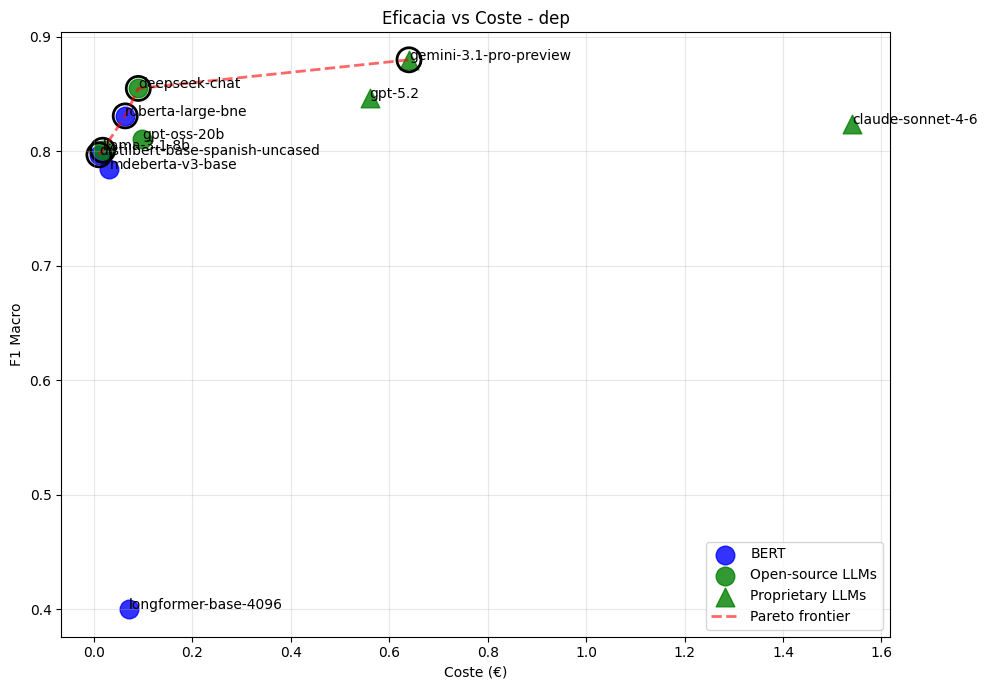
\includegraphics[width=0.9\linewidth]{figures/pareto_dep.png}
	\caption{Diagrama eficacia-coste y frontera de Pareto para la tarea de depresión.}
	\label{fig:pareto_dep}
\end{figure}

Como se observa en la Figura \ref{fig:pareto_dep}, la frontera de Pareto en la tarea de depresión está formada por DistilBERT, RoBERTa-large-BNE, Llama-3.1-8B, DeepSeek-Chat y Gemini 3.1 Pro. Esto refleja un escenario más equilibrado que en ansiedad, donde tanto modelos BERT como distintos tipos de LLMs ofrecen alternativas competitivas dependiendo del presupuesto disponible y del nivel de rendimiento deseado.

Dentro de los modelos tradicionales, RoBERTa-large-BNE vuelve a destacar por su excelente relación coste-rendimiento, alcanzando un F1 macro muy competitivo con un coste muy reducido frente a los LLMs propietarios. Del mismo modo, DistilBERT permanece en la frontera gracias a su coste prácticamente nulo, mientras que Llama-3.1-8B representa una opción intermedia de bajo coste con un rendimiento razonable. Entre los LLMs, DeepSeek-Chat ofrece una combinación especialmente eficiente al superar claramente a la mayoría de BERT sin un incremento excesivo de coste.

En el extremo de mayor rendimiento aparece Gemini 3.1 Pro, que constituye el punto de máxima eficacia dentro de la frontera de Pareto. Aunque su coste es notablemente superior, sigue formando parte de la frontera porque ningún otro modelo logra simultáneamente un mejor F1 macro con menor coste. Por el contrario, modelos como GPT-5.2, GPT-OSS-20B o Claude Sonnet 4.6 quedan dominados, ya que existen alternativas más baratas con rendimiento similar o incluso superior.


\section{Clasificación de TCA}

\subsection{Métricas principales y estabilidad predictiva}

\begin{table}[H]
	\centering
	\caption{Resultados principales en la tarea de clasificación de TCA}
	\label{tab:resultados_tca_metricas}
	\resizebox{\textwidth}{!}{
		\begin{tabular}{lccccc}
			\toprule
			\textbf{Modelo} & \textbf{F1 macro} & \textbf{Precision} & \textbf{Recall} & \textbf{MCC} & \textbf{TARa@5} \\
			\midrule
			DistilBETO & 0.920 [0.822, 0.980] & 0.920 [0.814, 0.977] & 0.920 [0.819, 0.978] & 0.840 [0.629, 0.958] & -- \\
			RoBERTa-large-BNE & 0.940 [0.838, 0.980] & 0.943 [0.859, 1.000] & 0.937 [0.816, 0.983] & 0.880 [0.669, 0.961] & -- \\
			mDeBERTa-v3 & 0.816 [0.694, 0.915] & 0.827 [0.696, 0.912] & 0.812 [0.692, 0.912] & 0.639 [0.385, 0.818] & -- \\
			Longformer & 0.362 [0.305, 0.407] & 0.284 [0.220, 0.343] & 0.500 [0.500, 0.500] & 0.000 [0.000, 0.000] & -- \\
			\midrule
			Llama 3.1 8B & 0.805 [0.760, 0.852] & 0.824 [0.782, 0.870] & 0.798 [0.754, 0.843] & 0.622 [0.534, 0.707] & 0.952 [0.924, 0.970] \\
			GPT-OSS-20B & 0.933 [0.901, 0.955] & 0.934 [0.901, 0.956] & 0.932 [0.900, 0.954] & 0.866 [0.801, 0.909] & 0.952 [0.922, 0.970] \\
			DeepSeek-V3.2 & 0.905 [0.869, 0.933] & 0.909 [0.873, 0.936] & 0.901 [0.866, 0.931] & 0.811 [0.739, 0.866] & 0.996 [0.976, 1.000] \\
			Claude Sonnet 4.6 & 0.936 [0.907, 0.961] & 0.934 [0.905, 0.959] & 0.939 [0.909, 0.963] & 0.873 [0.814, 0.921] & 0.996 [0.988, 1.000] \\
			GPT-5.2 & 0.963 [0.942, 0.982] & 0.963 [0.942, 0.981] & 0.963 [0.942, 0.982] & 0.927 [0.884, 0.963] & 0.992 [0.973, 0.998] \\
			Gemini 3.1 Pro & 0.951 [0.923, 0.970] & 0.953 [0.927, 0.972] & 0.949 [0.921, 0.970] & 0.902 [0.848, 0.940] & 0.998 [0.984, 1.000] \\
			\bottomrule
		\end{tabular}
	}
\end{table}

A diferencia de lo observado en ansiedad y depresión, en la tarea de clasificación de \ac{TCA} prácticamente todos los modelos alcanzan un rendimiento notablemente superior como se observa en la Tabla~\ref{tab:resultados_tca_metricas}. Esto sugiere que los patrones lingüísticos asociados a los trastornos de la conducta alimentaria presentan una mayor separabilidad respecto a la clase control, facilitando la discriminación automática incluso en modelos de menor capacidad.

El mejor resultado global corresponde a GPT-5.2, que alcanza el mayor F1-score macro (0.963), junto con los mejores valores de Precision, Recall y \ac{MCC} (0.927). Además, sus intervalos de confianza son especialmente sólidos y estrechos, lo que refuerza la estabilidad estadística de su rendimiento. Gemini 3.1 Pro se sitúa muy cerca, consolidando nuevamente el alto rendimiento de los modelos frontier en esta tarea.

Uno de los resultados más destacados aparece en RoBERTa-large-BNE, que obtiene un F1-score macro de 0.940, superando incluso a algunos \acp{LLM} como GPT-OSS-20B, DeepSeek-V3.2 o Claude Sonnet 4.6, y acercándose considerablemente a los dos mejores modelos propietarios. También resulta llamativo el comportamiento de DistilBETO, que pese a ser el modelo más pequeño y ligero, alcanza un F1 de 0.920, mostrando una competitividad muy superior a la observada en el resto de tareas binarias.

Dentro de los modelos open-source, GPT-OSS-20B vuelve a ser el mejor modelo, con un rendimiento prácticamente equivalente al de Claude Sonnet 4.6. En contraste, Llama 3.1 8B presenta aquí una diferencia mucho más acusada respecto al resto de \acp{LLM}, con un F1-score macro de 0.805, siendo el peor modelo de este grupo y acercándose más al rendimiento de mDeBERTa que al resto de modelos generativos.

Longformer vuelve a representar el caso más problemático, manteniendo el mismo patrón observado en tareas anteriores: Recall constante de 0.500 y \ac{MCC} igual a 0, lo que indica una predicción sistemática de la clase mayoritaria y una incapacidad para aprender una frontera de decisión útil bajo este escenario de desbalance.

En cuanto a la estabilidad inferencial, los valores de \ac{TARa@5} son elevados en todos los \acp{LLM}, confirmando una buena consistencia predictiva general. No obstante, vuelve a observarse que los modelos servidos mediante OpenRouter (Llama 3.1 8B y GPT-OSS-20B) presentan valores ligeramente inferiores, manteniendo el mismo patrón de menor estabilidad ya observado en el resto de tareas de clasificación binaria.

\subsection{Análisis de errores mediante matrices de confusión}

En el caso de la detección de Trastornos de la Conducta Alimentaria (TCA), la mayoría de modelos presentan un comportamiento notablemente más equilibrado que en ansiedad o depresión, con una diagonal dominante y una clara capacidad para discriminar entre usuarios control y casos positivos. Sin embargo, algunos modelos presentan patrones de error más relevantes: ciertos LLMs open-source muestran una mayor tendencia a clasificar falsamente casos positivos como controles (falsos negativos), mientras que otros priorizan la detección positiva a costa de aumentar falsos positivos.

Para ilustrar estas diferencias, en la Figura~\ref{fig:cm_tca} se muestran tres casos representativos: RoBERTa-large como mejor modelo BERT, GPT-5.2 como mejor modelo global y Llama-3.1-8B como ejemplo de modelo con mayor sesgo hacia falsos negativos. En el Anexo~\ref{anexo:mc_tca}, se incluye el conjunto completo de matrices de confusión de todos los modelos evaluados.

\begin{figure}[H]
	\centering
	
\includegraphics[width=\textwidth]{cm_tca.png}
	\caption{Matrices de confusión representativas en la tarea de clasificación de depresión}
	\label{fig:cm_tca}
\end{figure}

\begin{itemize}
	
	\item RoBERTa-large-BNE: Presenta una matriz altamente equilibrada, con un 96.6\% de acierto en la clase control y un 90.9\% en la clase positiva. El número de falsos positivos (3.4\%) y falsos negativos (9.1\%) es reducido y bastante simétrico, lo que explica su elevado F1 macro (0.940) y MCC (0.880). Este resultado demuestra que un modelo encoder especializado mediante fine-tuning puede competir directamente con LLMs mucho más grandes y costosos.
	
	\item GPT-5.2: Es el modelo con mejor comportamiento general, alcanzando un 96.9\% de acierto en controles y un 95.8\% en positivos. Tanto falsos positivos (3.1\%) como falsos negativos (4.2\%) son mínimos, reflejando una frontera de decisión muy robusta y estable. Esta matriz justifica su liderazgo en F1 macro (0.963) y MCC (0.927), siendo el modelo más preciso y equilibrado del estudio.
	
	\item Llama-3.1-8B: Aunque su rendimiento global sigue siendo competitivo, presenta un patrón de error clínicamente más problemático: un 31.5\% de los casos positivos reales son clasificados como controles. Esto implica una pérdida importante de sensibilidad diagnóstica, ya que aumenta el riesgo de no detectar usuarios con TCA. Aunque mantiene una buena precisión sobre la clase control (91.1\%), este sesgo reduce significativamente su F1 macro (0.805) y lo sitúa claramente por debajo de otros LLMs.
	
\end{itemize}

En conjunto, las matrices de confusión confirman que la tarea de detección de TCA es sustancialmente más separable que otras tareas binarias del estudio. Además, muestran que las diferencias entre modelos no se explican únicamente por el rendimiento global, sino por el equilibrio entre sensibilidad y especificidad, un aspecto especialmente relevante en aplicaciones clínicas de cribado automático.

\subsection{Comparación y significancia estadística entre modelos}

\begin{table}[H]
	\centering
	\small
	\begin{tabular}{llllll}
		\hline
		\textbf{Modelo A} & \textbf{Modelo B} & \textbf{Mean $\Delta$} & \textbf{Cohen's d} & \textbf{Effect size} & \textbf{\textit{p}} \\
		\hline
		RoBERTa-large-BNE & GPT-OSS-20B & -0.020 [-0.098, 0.039] & -0.637 & Medium & 0.914 \\
		RoBERTa-large-BNE & GPT-5.2 & -0.040 [-0.124, 0.000] & -1.468 & Large & 0.914 \\
		RoBERTa-large-BNE & Gemini 3.1 Pro & -0.020 [-0.099, 0.040] & -0.668 & Medium & 0.914 \\
		GPT-OSS-20B & GPT-5.2 & -0.020 [-0.099, 0.000] & -1.025 & Large & 0.914 \\
		GPT-OSS-20B & Gemini 3.1 Pro & 0.000 [-0.059, 0.060] & 0.001 & Negligible & 1.000 \\
		GPT-5.2 & Gemini 3.1 Pro & 0.020 [0.000, 0.118] & 0.973 & Large & 0.914 \\
		\hline
	\end{tabular}
	\caption{Comparación estadística mediante bootstrap pareado para la tarea de TCA.}
	\label{tab:bootstrap_tca}
\end{table}

Los resultados de la Tabla~\ref{tab:bootstrap_tca} muestran que las diferencias entre los mejores modelos en la tarea de TCA son considerablemente más reducidas que en ansiedad. Todas las comparaciones presentan diferencias medias de F1 macro muy pequeñas, generalmente próximas a cero, lo que indica un rendimiento muy similar entre los sistemas evaluados, como ya se vio anteriormente en la tabla de métricas principales~\ref{tab:resultados_tca_metricas}.

La comparación más favorable corresponde a RoBERTa-large-BNE frente a GPT-5.2, con $\Delta = -0.040 \quad [-0.124,\ 0.000]$ lo que sugiere una ligera ventaja de GPT-5.2 sobre el mejor modelo BERT. Sin embargo, el intervalo de confianza incluye el cero y el p-value ajustado es $p = 0.914$, por lo que no existe evidencia estadística suficiente para afirmar una superioridad robusta entre ambos modelos. Aunque el tamaño del efecto se clasifica como \textit{Large}, este resultado debe interpretarse con cautela debido a la reducida magnitud absoluta de la diferencia observada.

De forma similar, las comparaciones entre los propios LLMs muestran prácticamente un empate técnico. El caso más claro es GPT-OSS-20B frente a Gemini 3.1 Pro, donde $\Delta = 0.000 \quad [-0.059,\ 0.060]$ acompañado de $d = 0.001$
y un efecto \textit{Negligible}, confirma que ambos modelos presentan un comportamiento prácticamente idéntico en esta tarea.

En conjunto, los elevados p-values y los intervalos de confianza centrados en cero indican ausencia de diferencias estadísticamente significativas entre los mejores modelos. Esto sugiere que, en la detección de TCA, tanto los mejores BERT como los LLMs alcanzan niveles de rendimiento muy próximos, reduciendo notablemente la ventaja observada de los modelos más avanzados en otras tareas.

\subsection{Análisis rendimiento-coste}

\begin{figure}[H]
	\centering
	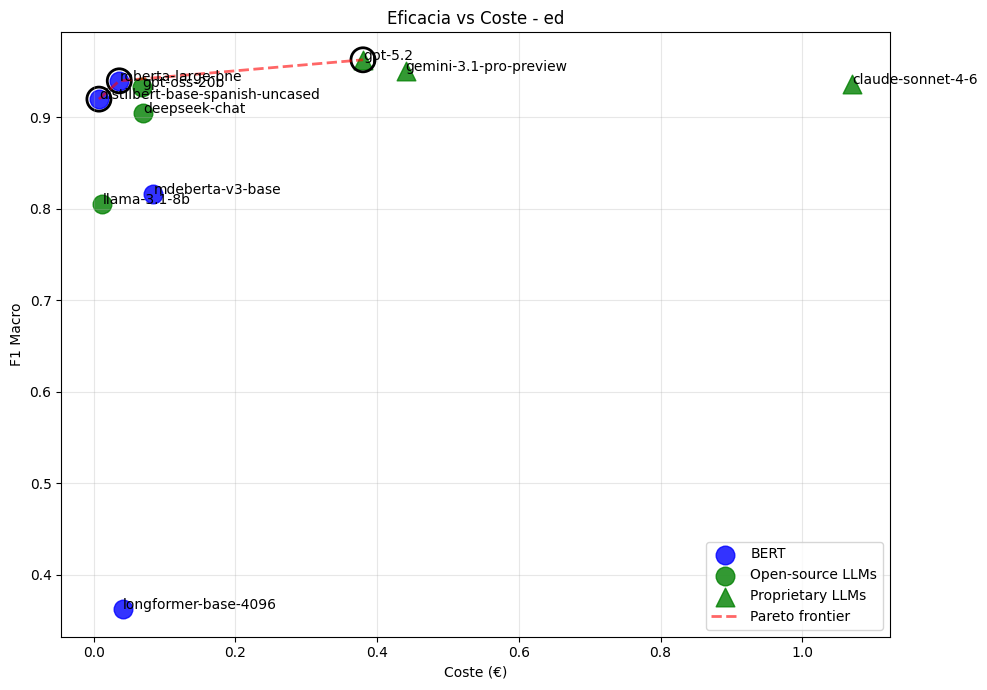
\includegraphics[width=0.9\linewidth]{figures/pareto_tca.png}
	\caption{Diagrama eficacia-coste y frontera de Pareto para la tarea de TCA.}
	\label{fig:pareto_tca}
\end{figure}

Como muestra la Figura \ref{fig:pareto_tca}, en la tarea de TCA la frontera de Pareto está formada principalmente por DistilBERT, RoBERTa-large-BNE y GPT-5.2. Esto indica que, a diferencia de lo observado en ansiedad, algunos modelos BERT mantienen una relación coste-rendimiento especialmente competitiva frente a los LLMs más avanzados.

En particular, RoBERTa-large-BNE destaca como uno de los modelos más eficientes del estudio, ya que alcanza un rendimiento muy próximo al de los mejores LLMs propietarios con un coste considerablemente inferior. De forma similar, DistilBERT permanece en la frontera gracias a su coste prácticamente nulo, constituyendo una alternativa especialmente atractiva cuando el presupuesto computacional es muy limitado. En el extremo opuesto, GPT-5.2 representa el punto de máximo rendimiento, aunque a costa de un incremento económico notable.

Por el contrario, modelos como GPT-OSS-20B, Gemini 3.1 Pro o Claude Sonnet 4.6 quedan fuera de la frontera de Pareto, ya que existen alternativas simultáneamente más baratas y con rendimiento igual o superior. Esto refuerza una conclusión importante en esta tarea: cuando las diferencias de F1 entre modelos son pequeñas, los modelos más costosos dejan de justificar su uso y opciones como RoBERTa-large-BNE ofrecen una eficiencia claramente superior.

\section{Clasificación multiclase}

\subsection{Métricas principales y estabilidad predictiva}

En la tarea de clasificación multiclase, el problema presenta una mayor complejidad al requerir distinguir entre cuatro etiquetas distintas: \texttt{0} (control), \texttt{1} (ansiedad), \texttt{2} (depresión) y \texttt{3} (\ac{TCA}). Esta configuración incrementa la dificultad respecto a los escenarios binarios anteriores, ya que el modelo no solo debe detectar la presencia de un trastorno, sino también discriminar correctamente entre diferentes categorías clínicas.

La Tabla~\ref{tab:resultados_multiclase_metricas} recoge los resultados principales obtenidos en esta tarea. Como puede observarse, el rendimiento general desciende respecto a las tareas binarias, especialmente en los \acp{LLM}, mientras que algunos modelos BERT mantienen un comportamiento notablemente competitivo.

\begin{table}[H]
	\centering
	\caption{Resultados principales en la tarea de clasificación multiclase}
	\label{tab:resultados_multiclase_metricas}
	\resizebox{\textwidth}{!}{
		\begin{tabular}{lccccc}
			\toprule
			\textbf{Modelo} & \textbf{F1 macro} & \textbf{Precision} & \textbf{Recall} & \textbf{MCC} & \textbf{TARa@5} \\
			\midrule
			DistilBETO & 0.818 [0.758, 0.865] & 0.844 [0.778, 0.884] & 0.834 [0.775, 0.875] & 0.744 [0.673, 0.807] & -- \\
			RoBERTa-large-BNE & 0.842 [0.778, 0.890] & 0.846 [0.774, 0.895] & 0.845 [0.780, 0.888] & 0.786 [0.703, 0.846] & -- \\
			mDeBERTa-v3 & 0.790 [0.725, 0.846] & 0.822 [0.762, 0.867] & 0.779 [0.705, 0.838] & 0.709 [0.628, 0.779] & -- \\
			Longformer & 0.770 [0.706, 0.824] & 0.778 [0.708, 0.833] & 0.775 [0.705, 0.826] & 0.674 [0.588, 0.747] & -- \\
			\midrule
			Llama 3.1 8B & 0.729 [0.706, 0.752] & 0.732 [0.710, 0.753] & 0.783 [0.763, 0.801] & 0.667 [0.638, 0.694] & 0.837 [0.822, 0.846] \\
			GPT-OSS-20B & 0.787 [0.761, 0.810] & 0.792 [0.766, 0.816] & 0.799 [0.774, 0.820] & 0.715 [0.683, 0.744] & 0.847 [0.837, 0.856] \\
			DeepSeek-V3.2 & 0.802 [0.780, 0.822] & 0.825 [0.801, 0.842] & 0.801 [0.777, 0.821] & 0.725 [0.697, 0.751] & 0.883 [0.877, 0.891] \\
			GPT-5.2 & 0.789 [0.764, 0.810] & 0.802 [0.779, 0.823] & 0.819 [0.799, 0.835] & 0.725 [0.696, 0.750] & 0.868 [0.860, 0.878] \\
			Claude Sonnet 4.6 & 0.785 [0.761, 0.806] & 0.797 [0.776, 0.818] & 0.827 [0.810, 0.844] & 0.731 [0.705, 0.758] & 0.878 [0.872, 0.885] \\
			Gemini 3.1 Pro & 0.864 [0.845, 0.882] & 0.855 [0.834, 0.874] & 0.877 [0.859, 0.893] & 0.809 [0.783, 0.834] & 0.885 [0.878, 0.892] \\
			\bottomrule
		\end{tabular}
	}
\end{table}

El mejor resultado global corresponde de forma clara a Gemini 3.1 Pro, que alcanza el mayor F1-score macro (0.864) y el mejor valor de \ac{MCC} (0.809), situándose por encima del resto de modelos con una diferencia apreciable. También resulta destacable RoBERTa-large-BNE, que con un F1 de 0.842 supera a todos los \acp{LLM} excepto Gemini, confirmando nuevamente el excelente comportamiento de este modelo encoder en tareas de clasificación supervisada. Del mismo modo, DistilBETO sorprende positivamente al alcanzar un F1 de 0.818, muy cercano a RoBERTa y superior incluso al de varios modelos generativos mucho más grandes.

Longformer muestra aquí un comportamiento diferente al observado en las tareas binarias. Aunque sigue situándose entre los modelos de menor rendimiento, ya no presenta el patrón degenerado de predecir únicamente la clase mayoritaria, sino que consigue discriminar entre varias clases, reflejado en un \ac{MCC} de 0.674. Aun así, su rendimiento continúa claramente por debajo de los mejores modelos. En el extremo opuesto, Llama 3.1 8B vuelve a ser el peor \ac{LLM} con diferencia, obteniendo el F1-score más bajo de todo el grupo generativo.

En cuanto a la estabilidad predictiva, los valores de \ac{TARa@5} son sensiblemente inferiores a los observados en las tareas binarias, donde habitualmente se situaban muy próximos a 1. Esta reducción era esperable, ya que al aumentar el número de etiquetas posibles también aumenta la dificultad de mantener exactamente la misma predicción en múltiples ejecuciones independientes. Aun así, los modelos propietarios siguen mostrando una mayor consistencia que los modelos servidos mediante OpenRouter, manteniéndose el mismo patrón observado en el resto del trabajo.

\subsection{Análisis de errores mediante matrices de confusión}

En la tarea de clasificación multiclase, la interpretación de las matrices de confusión resulta más compleja que en los problemas binarios anteriores, ya que los errores no pueden resumirse simplemente en términos de falsos positivos y falsos negativos.

De forma general, se observa un patrón claro de confusión entre las clases 0, 1 y 2, que corresponden respectivamente a control, ansiedad y depresión. Estas tres categorías concentran la mayor parte de los errores y tienden a confundirse entre sí de forma recurrente, especialmente entre ansiedad y depresión, lo que sugiere una mayor proximidad semántica entre ellas. Por el contrario, la clase 3 (TCA) presenta porcentajes de acierto considerablemente más altos y un menor nivel de confusión con el resto de clases.

Este comportamiento ya se anticipaba en la Figura~\ref{fig:embeddings_visualization} de visualización de embeddings, donde puede observarse que las clases 0, 1 y 2 aparecen más cercanas en el espacio semántico, con regiones de solapamiento más evidentes. En cambio, la clase 3 se encuentra más separada del resto, formando un grupo más diferenciado. Esta mayor separación facilita su identificación por parte de los modelos y explica por qué suele ser la clase mejor clasificada en la mayoría de matrices de confusión.

La Figura \ref{fig:cm_multi} muestra tres casos representativos: RoBERTa-large-BNE como mejor modelo BERT, GPT-5.2 como ejemplo de LLM con alto rendimiento pero cierta asimetría entre clases, y Gemini 3.1 Pro como el modelo más equilibrado globalmente. El conjunto completo de matrices de confusión para esta tarea se incluyen en el Anexo~\ref{anexo:mc_multi}.

\begin{figure}[H]
	\centering
	
\includegraphics[width=\linewidth]{cm_multi.png}
	\caption{Matrices de confusión representativas para la tarea de clasificación multiclase.}
	\label{fig:cm_multi}
\end{figure}

\begin{itemize}
	
	\item RoBERTa-large-BNE: presenta una matriz bastante sólida en las clases 0, 1 y 3, con porcentajes de acierto cercanos o superiores al 90\%. Sin embargo, la clase 2 resulta considerablemente más difícil, descendiendo hasta el 66.0\% y mostrando confusiones frecuentes con las clases 0 y 1.
	
	\item GPT-5.2: destaca especialmente en la clase 1 y la clase 3, alcanzando un 95.3\% y 98.6\% de acierto respectivamente, lo que refleja una gran capacidad para identificar correctamente estas categorías. No obstante, su rendimiento en la clase 0 desciende notablemente (57.3\%), mostrando una mayor tendencia a confundirla con otras clases, especialmente con la clase 1.
	
	\item Gemini 3.1 Pro: muestra la matriz más equilibrada del estudio, manteniendo valores altos y homogéneos en todas las clases (81.8\%, 88.5\%, 83.9\% y 96.5\%). A diferencia de otros modelos, no presenta una clase claramente problemática, lo que explica su excelente rendimiento global y confirma una mayor estabilidad predictiva en escenarios multiclase.
	
\end{itemize}

\subsection{Comparación y significancia estadística entre modelos}

\begin{table}[H]
	\centering
	\small
	\begin{tabular}{llllll}
		\hline
		\textbf{Modelo A} & \textbf{Modelo B} & \textbf{Mean $\Delta$} & \textbf{Cohen's d} & \textbf{Effect size} & \textbf{\textit{p}} \\
		\hline
		RoBERTa-large-BNE & DeepSeek-Chat & 0.039 [-0.062, 0.130] & 0.775 & Medium & 0.818 \\
		RoBERTa-large-BNE & Gemini 3.1 Pro & 0.023 [-0.062, 0.108] & 0.513 & Medium & 0.818 \\
		RoBERTa-large-BNE & GPT-5.2 & 0.044 [-0.052, 0.164] & 0.754 & Medium & 0.818 \\
		DeepSeek-Chat & Gemini 3.1 Pro & -0.016 [-0.092, 0.062] & -0.411 & Small & 0.818 \\
		DeepSeek-Chat & GPT-5.2 & 0.004 [-0.091, 0.089] & 0.100 & Negligible & 0.934 \\
		Gemini 3.1 Pro & GPT-5.2 & 0.021 [-0.075, 0.105] & 0.444 & Small & 0.818 \\
		\hline
	\end{tabular}
	\caption{Comparación estadística mediante bootstrap pareado para la tarea de clasificación multiclase.}
	\label{tab:bootstrap_multi}
\end{table}

A diferencia de las tareas binarias, en clasificación multiclase las diferencias entre los mejores modelos son especialmente reducidas. Sin embargo, al igual que ocurría en las tareas anteriores, todas las comparaciones presentan valores de \textit{Mean $\Delta$} pequeños y, además, todos los intervalos de confianza incluyen el valor cero, lo que indica ausencia de evidencia suficiente para afirmar una superioridad consistente entre modelos.

Por ejemplo, la comparación entre roberta-large-bne y gpt-5.2 presenta la mayor diferencia observada ($\Delta = 0.044 \quad [-0.052,\ 0.164]$) lo que sugiere una ligera ventaja para el modelo BERT. Sin embargo, el intervalo de confianza atraviesa el cero y el \textit{p-value} ajustado es elevado ($p = 0.818$) por lo que dicha diferencia no puede considerarse estadísticamente significativa.

Aunque algunas comparaciones presentan valores de Cohen’s \(d\) clasificados como \textit{Medium}, la amplitud de los intervalos de confianza y los elevados \textit{p-values} impiden consolidar estas diferencias como robustas desde el punto de vista estadístico. Esto sugiere que las pequeñas variaciones observadas en F1 macro pueden atribuirse principalmente a la variabilidad propia del conjunto de evaluación.

\subsection{Análisis rendimiento-coste}

\begin{figure}[H]
	\centering
	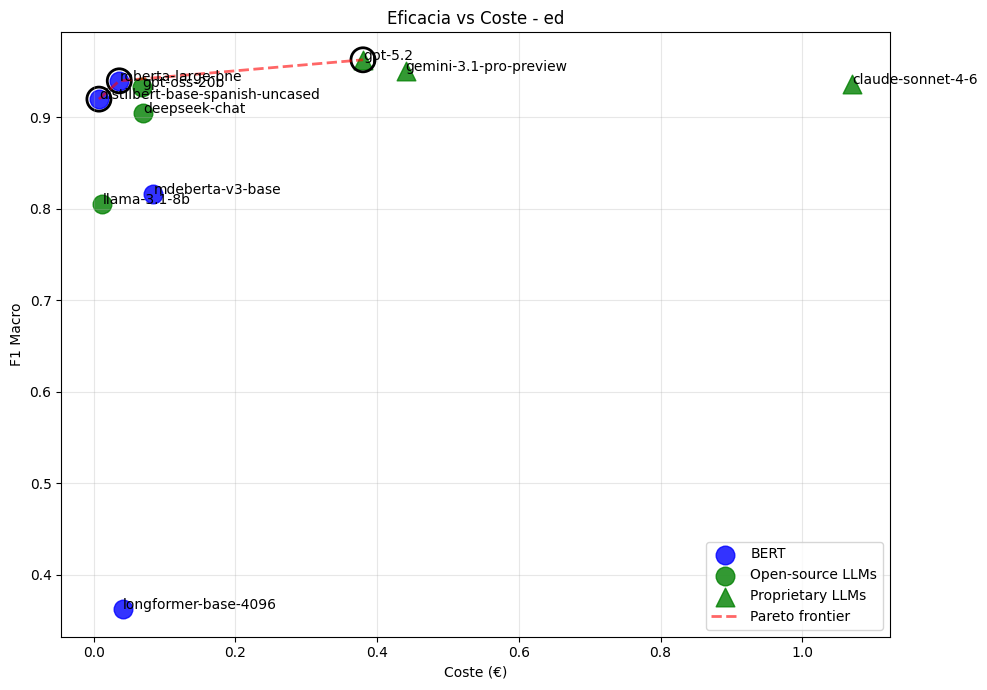
\includegraphics[width=0.9\linewidth]{figures/pareto_tca.png}
	\caption{Diagrama eficacia-coste y frontera de Pareto para la tarea de TCA.}
	\label{fig:pareto_multi}
\end{figure}

La Figura \ref{fig:pareto_multi} muestra que, incluso en la tarea multiclase, la frontera de Pareto vuelve a estar formada por roberta-large-bne, distilbert-base-spanish-uncased y gemini-3.1-pro-preview, exactamente los mismos modelos que ya aparecían en depresión y TCA. Esto refuerza la consistencia del análisis coste-rendimiento y sugiere que estos tres modelos representan las opciones más eficientes cuando se consideran simultáneamente rendimiento predictivo y coste computacional.

Dentro de esta frontera, roberta-large-bne destaca como una de las alternativas más equilibradas, ya que alcanza un F1 macro muy competitivo con un coste extremadamente bajo. DistilBERT presenta un coste aún menor, aunque con una ligera pérdida de rendimiento. Por su parte, gemini-3.1-pro-preview obtiene el mejor rendimiento absoluto de la tarea, pero a cambio de un incremento considerable en el coste, situándose como la opción más potente aunque menos eficiente económicamente.

Un aspecto especialmente relevante en esta tarea es el comportamiento de claude-sonnet-4-6. A diferencia de las tareas binarias anteriores, donde su elevado coste se acompañaba de un rendimiento competitivo, en clasificación multiclase presenta un F1 macro relativamente bajo pese a ser el modelo más caro con diferencia. Esto lo sitúa claramente fuera de la frontera de Pareto y reduce notablemente su atractivo práctico frente a alternativas más baratas y con mejor rendimiento, como gemini-3.1-pro-preview o incluso varios modelos open-source.

En conjunto, estos resultados indican que en clasificación multiclase el aumento de coste no garantiza necesariamente una mejora de rendimiento proporcional. De hecho, modelos más ligeros como roberta-large-bne continúan ofreciendo una relación rendimiento-coste muy favorable, mientras que algunos LLMs propietarios pierden eficiencia relativa al enfrentarse a una tarea donde la separación entre clases resulta considerablemente más compleja.

\section{Entorno experimental}
\label{sec:entorno-experimental}

Blah, blah, blah.


\subsection{Bases de datos utilizadas}
\label{sec:bases-de-datos-1}

Blah, blah, blah.


\subsection{Métricas de calidad}
\label{sec:metricas-de-calidad}

Blah, blah, blah.

En la tabla\ref{pruebaCalc2LaTeX} pongo un ejemplo del uso del conversor de libreoffice a \LaTeX{} (cortesía de Roberto Chamorro). Para usarlo tienes que importar la macro que encontrarás en el directorio \texttt{Tools/calc2latex//calc2latex\_024\_eur\_latex}\footnote{Para ello sigue el proceso de importación que se describe en \url{http://ask.libreoffice.org/en/question/35598/where-are-lo-basic-macros-stored/}, importando Cals y cuando ejecutes la macro hazlo por el punto de entrada \texttt{Main}, después de seleccionar el rango de celdas de la tabla.}

\input{Tools/calc2latex/sample.tex}


\subsection{Estrategia y metodología de experimentación}
\label{sec:estr-y-metod}

Blah, blah, blah.


\section{Resultados experimentales}
\label{sec:result-experim}

A continuación, se muestra un ejemplo de tabla simple (ver tabla \ref{tab:table1}).

\begin{table}
  % increase table row spacing, adjust to taste
  \renewcommand{\arraystretch}{1.3}
  \caption{Comparativa.}
  \label{tab:table1}
  \begin{center}
    % Some packages, such as MDW tools, offer better commands for making tables than the plain LaTeX2e tabular which is used here.
    \begin{tabular}{|c|c|c|}
      \hline
      Method & Training Time & Man-Work (\%)\\
      \hline
      Propagation model & $<$ 30 sec & 5\\
      \hline
      Manual & 9 h 30 min & 24\\
      \hline
      Automatic & 2 h & 10 8\\
      \hline
    \end{tabular}
  \end{center}
\end{table}

Cuando las tablas ocupan más de un página se debe utilizar un tipo especial de tablas denominado \texttt{longtable}. A continuación, se muestra un ejemplo del mismo (ver tabla \ref{table2}).

\begin{center}
	\begin{longtable}{|c|c|c|c|}
    \caption[Resultados de la correlación cruzada.]{Resultados de la correlación cruzada.} \label{table2} \\
    
    \hline \multicolumn{1}{|c|}{\textbf{Posición Real}} & \multicolumn{1}{c|}{\textbf{Posición estimada}} & \multicolumn{1}{c|}{\textbf{Coef. Correlación}} & \multicolumn{1}{c|}{\textbf{Acierto/Fallo}} \\ \hline 
    \endfirsthead
    
    \multicolumn{4}{c}%
    {{\bfseries \tablename\ \thetable{} -- continúa en la página anterior}} \\
    \hline \multicolumn{1}{|c|}{\textbf{Posición Real}} & \multicolumn{1}{c|}{\textbf{Posición estimada}} & \multicolumn{1}{c|}{\textbf{Coef. Correlación}} & \multicolumn{1}{c|}{\textbf{Acierto/Fallo}} \\ \hline 
    \endhead
    
    \hline \multicolumn{4}{|r|}{{Continúa en la página siguiente}} \\ \hline
    \endfoot

    \hline \hline
    \endlastfoot
    
    \hline	2P0	&	2P0	&	0,004954	&	A	\\
    \hline	2P1	&	2P4	&	0,005752	&	F	\\
    \hline	2P2	&	2P2	&	0,005461	&	A	\\
    \hline	2P3	&	2P0	&	0,004634	&	F	\\
    \hline	2P5	&	2P4	&	0,005991	&	F	\\
    \hline	2P6	&	2P16	&	0,004410	&	F	\\
    \hline	2P7	&	3P9	&	0,008038	&	F	\\
    \hline	2P8	&	3P9	&	0,003753	&	F	\\
    \hline	2P9	&	2P7	&	0,004908	&	F	\\
    \hline	2P10	&	2P10	&	0,007273	&	A	\\
    \hline	2P14	&	2P16	&	0,006485	&	F	\\
    \hline	2P15	&	2P15	&	0,004932	&	A	\\
    \hline	2P16	&	2P16	&	0,006237	&	A	\\
    \hline	2P17	&	2P15	&	0,005110	&	F	\\
    \hline	2P18	&	3P18	&	0,006235	&	F	\\
    \hline	2P19	&	3P18	&	0,004827	&	F	\\
    \hline	2P20	&	2P20	&	0,006877	&	A	\\
    \hline	2P22	&	3P18	&	0,003048	&	F	\\
    \hline	2P24	&	2P24	&	0,006833	&	A	\\
    \hline	2P25	&	2P25	&	0,004875	&	A	\\
    \hline	2P26	&	2P31	&	0,005511	&	F	\\
    \hline	2P27	&	2P28	&	0,004590	&	F	\\
    \hline	2P30	&	2P31	&	0,005576	&	F	\\
    \hline	2P31	&	2P31	&	0,007213	&	A	\\
    \hline	2P32	&	2P35	&	0,003340	&	F	\\
    \hline	2P34	&	2P34	&	0,004128	&	A	\\
    \hline	2P36	&	2P35	&	0,003329	&	F	\\
    \hline	2P37	&	2P37	&	0,003468	&	A	\\
    \hline	2P39	&	2P38	&	0,002577	&	F	\\
    \hline	2P40	&	2P43	&	0,004303	&	F	\\
    \hline	2P41	&	2P41	&	0,001573	&	A	\\
    \hline	2P42	&	2P41	&	0,000846	&	F	\\
    \hline	2P44	&	2P44	&	0,002732	&	A	\\
    \hline	2P45	&	23P45	&	0,001958	&	F	\\
    \hline	2P47	&	2P34	&	0,002869	&	F	\\
    \hline	2P48	&	2P43	&	0,004569	&	F	\\
    \hline	2P49	&	3P51	&	0,001374	&	F	\\
    \hline	2P50	&	2P34	&	0,002274	&	F	\\
    \hline	2P51	&	2P63	&	0,003931	&	F	\\
    \hline	2P52	&	2P55	&	0,003537	&	F	\\
    \hline	2P53	&	3P56	&	0,003126	&	F	\\
    \hline	2P54	&	2P67	&	0,005560	&	F	\\
    \hline	2P56	&	2P55	&	0,002817	&	F	\\
    \hline	2P57	&	2P67	&	0,006168	&	F	\\
    \hline	2P58	&	2P58	&	0,005278	&	A	\\
    \hline	2P60	&	3P66	&	0,004966	&	F	\\
    \hline	2P61	&	3P61	&	0,004748	&	A	\\
    \hline	2P64	&	2P67	&	0,005342	&	F	\\
    \hline	2P66	&	2P4	&	0,004172	&	F	\\
    \hline	2P67	&	2P67	&	0,005706	&	A	\\
    \hline	3P0	&	3P0	&	0,003674	&	A	\\
    \hline	3P61	&	2P61	&	0,003263	&	F	\\
    \hline	3P64	&	2P67	&	0,003484	&	F	\\
    \hline	3P65	&	2P67	&	0,002975	&	F	\\
    \hline	3P66	&	2P58	&	0,005029	&	F	\\
    \hline	3P67	&	3P67	&	0,003714	&	A	\\
	\end{longtable}
\end{center}

En algunas ocasiones, también resulta útil emplear el entorno
\texttt{subfigure} para añadir múltiples imágenes dentro de la misma
figura. A continuación, se muestra un ejemplo del uso en la figura
\ref{fig:fig3}. También se pueden referenciar las sub-figuras de forma
individual, por ejemplo la sub-figura \ref{fig:fig3b} (usando un método
de cita), o bien la sub-figura \ref{fig:fig3}.\subref{fig:fig3b} (usando
otro alternativo).

% For this to work you need to (in preamble.tex):
% - remove \usepackage{subfig}
% - add \usepackage{caption}
% - add \usepackage{subcaption}
\begin{figure}
  \centering
  \begin{subfigure}[b]{0.3\textwidth}
    
\includegraphics[width=\textwidth]{Figure2}
    \caption{Mean Entropy.}
    \label{fig:fig3a}
  \end{subfigure}%
  ~ %add desired spacing between images, e. g. ~, \quad, \qquad etc.
  % (or a blank line to force the subfigure onto a new line)
  \begin{subfigure}[b]{0.3\textwidth}
    
\includegraphics[width=\textwidth]{Figure3}
    \caption{Error Percentage.}
    \label{fig:fig3b}
  \end{subfigure}
  \caption{Optimal trames number in the training data set.}
  \label{fig:fig3}
\end{figure}

La figura~\ref{fig:LIdiapRoom} muestra otro ejemplo con referencias a las subfigures en el caption principal.

\begin{figure}
  \centering
  \begin{subfigure}[b]{0.30\textwidth}
    
\includegraphics[width=\textwidth]{roomlayout2}
    \caption{}
    \label{fig:RoomLayout}
  \end{subfigure}%
  \qquad \qquad %add desired spacing between images, e. g. ~, \quad, \qquad, \hfill etc.
  % (or a blank line to force the subfigure onto a new line)
  \begin{subfigure}[b]{0.425\textwidth}
    
\includegraphics[width=\textwidth]{idiap-seq45-cam2.jpg}
    \caption{}
    \label{fig:RoomPicture}
  \end{subfigure}
  \caption{Idiap Smart Meeting Room for AV16.3 recordings. (\protect\subref{fig:RoomLayout}) Room layout showing the centered table, and the microphones arranged in two circular arrays. (\protect\subref{fig:RoomPicture}) Sample of recorded video frame showing the arrays area. %\vspace{-0.3cm}
  }
  \label{fig:LIdiapRoom}
\end{figure}

Os incluimos a continuación un párrafo de un artículo en el que hacemos referencia a varias figuras y subfiguras:

\emph{The IDIAP Meeting Room (shown in figure~\ref{fig:LIdiapRoom}) is a $8.2m \times 3.6m \times 2.4m$ rectangular space containing a centrally located $4.8m \times 1.2m$ rectangular table, on top of which two circular microphone arrays of $10 cm$ radius are located, each of them composed by 8 microphones. The centers of the two arrays are separated by $80 cm$ and the origin of coordinates is located in the middle point between the two arrays. The arrays can be also seen in figures~\ref{fig:simureal_positions}.\subref{fig:Simulated_positions}, ~\ref{fig:simureal_positions}.\subref{fig:real_positions_short}, and ~\ref{fig:simureal_positions}.\subref{fig:real_positions_long}, in which only the relevant section of the room is displayed, each one showing different scenarios that were used in the experiments. A detailed description of the meeting room can be found in~\cite{moore2002}.}

\begin{figure}
  \centering
  \begin{subfigure}[t]{0.3\textwidth}
    
\includegraphics[width=\textwidth]{angular2-short-improved}
    \caption{For validation\\with simulated data.}
    \label{fig:Simulated_positions}
  \end{subfigure}
~%add desired spacing between images, e. g. ~, \quad, \qquad,
  % \hfill etc.
  % (or a blank line to force the subfigure onto a new line)
  \begin{subfigure}[t]{0.3\textwidth}
    
\includegraphics[width=\textwidth]{positions1-short-improved}
    \caption{For validation\\with real data and microphone pairs with $20~cm$ spacing.}
    \label{fig:real_positions_short}
  \end{subfigure}
  ~
  \begin{subfigure}[t]{0.3\textwidth}
    
\includegraphics[width=\textwidth]{positions2-short-improved}
    \caption{For validation\\with real data and microphone pairs with
      $82.46~cm$ spacing.}
    \label{fig:real_positions_long}
  \end{subfigure}
  \caption{Geometrical details for the experiments carried out. Only the
    relevant section of the room is shown, and microphone pairs are
    connected by solid lines.}
  \label{fig:simureal_positions}
\end{figure}

En la figura~\ref{fig:Sim_angles} mostramos un ejemplo de varias
figuras organizadas de forma un poco más complejo.

\begin{figure}
  \centering
  \begin{subfigure}[b]{0.3\textwidth}
    
\includegraphics[width=\textwidth]{Sim_seg025_ang090}
    \caption{$0^{\circ}$}
    \label{fig:Sim_ang090}
  \end{subfigure}
  % add desired spacing between images, e. g. ~, \quad, \qquad etc.
  % (or a blank line to force the subfigure onto a new line)

  \begin{subfigure}[b]{0.3\textwidth}
    
\includegraphics[width=\textwidth]{Sim_seg025_ang108}
    \caption{$18^{\circ}$}
    \label{fig:Sim_ang108}
  \end{subfigure}
  % add desired spacing between images, e. g. ~, \quad, \qquad etc.
  % (or a blank line to force the subfigure onto a new line)
  \begin{subfigure}[b]{0.3\textwidth}
    
\includegraphics[width=\textwidth]{Sim_seg025_ang126}
    \caption{$36^{\circ}$}
    \label{fig:Sim_ang126}
  \end{subfigure}
  % add desired spacing between images, e. g. ~, \quad, \qquad etc.
  % (or a blank line to force the subfigure onto a new line)
  \begin{subfigure}[b]{0.3\textwidth}
    
\includegraphics[width=\textwidth]{Sim_seg025_ang144}
    \caption{$54^{\circ}$}
    \label{fig:Sim_ang144}
  \end{subfigure}
  % add desired spacing between images, e. g. ~, \quad, \qquad etc.
  % (or a blank line to force the subfigure onto a new line)

  \begin{subfigure}[b]{0.3\textwidth}
    
\includegraphics[width=\textwidth]{Sim_seg025_ang162}
    \caption{$72^{\circ}$}
    \label{fig:Sim_ang162}
  \end{subfigure}

  \caption{Comparison between the steered power response generated by the model (solid line) and that calculated using simulated waveforms in the AV16.3 environment (stems). Results for the speaker in given angles and the array steered from -90º to +90º are shown.}
  \label{fig:Sim_angles}
\end{figure}

También es posible incluir el código de una figura en un fichero \texttt{.tex} independiente (para hacer más legible el código del documento principal). Un ejemplo lo tenéis a continuación, incluyendo el texto en inglés del documento original:

\emph{Figure~\ref{fig:SRPvsPatternSelected} includes the results of the comparison, for several speaker positions (1, 2, 4, 6, 8 and 16, emphasized in figure~\ref{fig:simureal_positions}.\subref{fig:real_positions_short}), and selected to provide different acoustic situations, both in terms of distance and angular position with respect to the arrays. All the graphics show the acoustic power map (predicted or calculated) for a regular two-dimensional grid of $10~cm$. The plot is provided from a top view of the room, spanning the full plan at a height of $61~cm$ above the microphone arrays (this height was the ground truth one for sequence 01). For each speaker position shown, three graphics are plotted:}

\begin{itemize}
  \item \emph{The graphics on the left show the SRP-PHAT acoustic power maps generated by the proposed model (for example, the left graphic in figure~\ref{fig:SRPvsPatternSelected}.\subref{fig:SRPvsModel_Fo1500_position1} for position 1).}
  \item \emph{The graphics in the middle show the real SRP-PHAT acoustic power maps calculated using the real acoustic waveforms (for example, the middle graphic in figure~\ref{fig:SRPvsPatternSelected}.\subref{fig:SRPvsModel_Fo1500_position1} for position 1), for a single selected frame.}
  \item \emph{The graphics on the right show the average real SRP-PHAT acoustic power maps, averaging for all the frames in which the user was in the given position (for example, the right graphic in figure~\ref{fig:SRPvsPatternSelected}.\subref{fig:SRPvsModel_Fo1500_position1} for position 1).}
\end{itemize}

\emph{The green point represents the real (ground truth) speaker position, and the black dots represent the positions of the four microphones used. The hyperbolic shapes found in the figure are consistent with the fact that the place of points with equal acoustic power value, for a given microphone pair, is a hyperbola (in our two-dimensional case, being a hyperboloid of revolution in the three-dimensional case).}

\emph{From figure~\ref{fig:SRPvsPatternSelected}, it can clearly be seen that, again, the predictions closely match the results with real data for the different acoustic conditions, even when the simulations are using fixed and frequency independent average reflection coefficients, and that the acoustic model is based on the simplistic image method model.}

\input{chapters/figure-ComparisonMap} 

\begin{wrapfigure}{r}{0.5\textwidth} 
\vspace{-20pt}
  \begin{center}
    
\includegraphics[width=0.4\textwidth]{Figure1}
    \caption{Ejemplo de figura con wrapfigure.}
    \label{fig:wrapfigure1}
  \end{center}
  \vspace{-20pt}
  \vspace{1pt}
\end{wrapfigure} 

Otra posibilidad es utilizar el entorno \texttt{wrapfig} para hacer que el texto bordee a las figuras, como en la figura~\ref{fig:wrapfigure1}. Añado ahora unas líneas de loren ipsum para que lo veáis bien. \lipsum[1-1]

% \lipsum[1-4]
% \begin{wrapfigure}{R}{5cm}
% \centering
% \rule{3cm}{7cm}
% \end{wrapfigure}
% \lipsum[1-6]

Incluso podemos poner una tabla ``apaisada'', como en la \ref{tab:tablas2006}, donde se muestra un resumen de los resultados obtenidos en una serie de experimentos de localización de locutores.

\clearpage
% \begin{table}[H]\centering
\begin{sidewaystable}[hbtp]
  \begin{center}

    \begin{tabular}{||l|c|c|c|c|c||}
      \hline \hline
      & UKA & ITC & AIT & UPC & IBM\\
      \hline
      \hline
      Pcor & $57.0\pm1.4\%$ & $84.0\pm3.3\%$ & $47.0\pm3.1\%$ & $20.0\pm2.5\%$ & $67.0\pm2.9\%$ \\
      \hline
      Bias fine (x:y:z) [mm] & $20:-42:-75$ & $45:27:-41$ & $-27:-77:-40$ & $-59:112:52$ & $91:-69:-38$ \\
      \hline
      Bias fine+gross (x,y,z) [mm] & $735:-93:-258$ & $67:439:-134$ & $17:-402:-118$ & $-141:255:39$ & $474:-141:-14$ \\
      \hline
      AEE fine [mm] = MOTP & $210$ & $130$ & $266$ & $344$ & $228$ \\
      \hline
      Fine+gross [mm] & $1201$ & $632$ & $1006$ & $1188$ & $884$ \\
      \hline
      Loc. frames & $5035$ & $22$ & $995$ & $977$ & $1023$ \\
      \hline
      Ref. duration (s) & $6287.0$ & $596.0$ & $1143.0$ & $1180.0$ & $1194.0$ \\
      \hline \hline
    \end{tabular}
    \caption{Resultados TEST CLEAR 2006.}
    \label{tab:tablas2006}
  \end{center}
\end{sidewaystable}
% \end{table}


\section{Conclusiones}
\label{sec:conclusiones-resultados}

Blah, blah, blah.


%%% Local Variables:
%%% TeX-master: "../book"
%%% End:
